\chapter{Semi-Global Kuranishi Structure and Full Contact Homology}
\label{b3}
\abstract{In this lecture, we introduce the semi-global Kuranishi structure. We explore its application in relation to obstruction bundle gluing, including computations of simple examples. The discussion will culminate in the rigorous definition of full contact homology, facilitated by the semi-global Kuranishi structure.}

\section{Introduction}
Suppose $(W,\,d\alpha)$ is an exact symplectic manifold with $\partial W=W_+ + W_-, \alpha|_{W_\pm}=W_{\pm}$, and $J$ an almost complex surface on $\hat{W}$. To count $\text{ind}=0$ $J$-holomorphic cylinders, we obtain a chain map
\[
\Phi: c_*(W_+, \alpha_+, J_+) \to c_*(w_-, \alpha_-, J_-)
\]

Given a 1-parameter family of this data $(W^2, \,d\alpha^2, J^2)$ we want $ \Phi_0 < \Phi_1$ to induce the same map on homology:
\[
\mathcal{M}(\gamma_+, \gamma_-) = \bigsqcup_\iota \{ \iota \}\times \mathcal{M}_{J^2}^{\text{ind}=0} (\gamma_+, \gamma_-).
\]

We want to show that there exists a linear map $K: c_+(W_+, \alpha_+, J_+) \to c_*(W_-, \alpha_-, J_-)$ such that $\Phi_0-\Phi_1 = K\partial + \partial K$.

We have:
\newpage
\vspace{-20pt}
\begin{center}
    \begin{figure}[htbp]
  \centering
  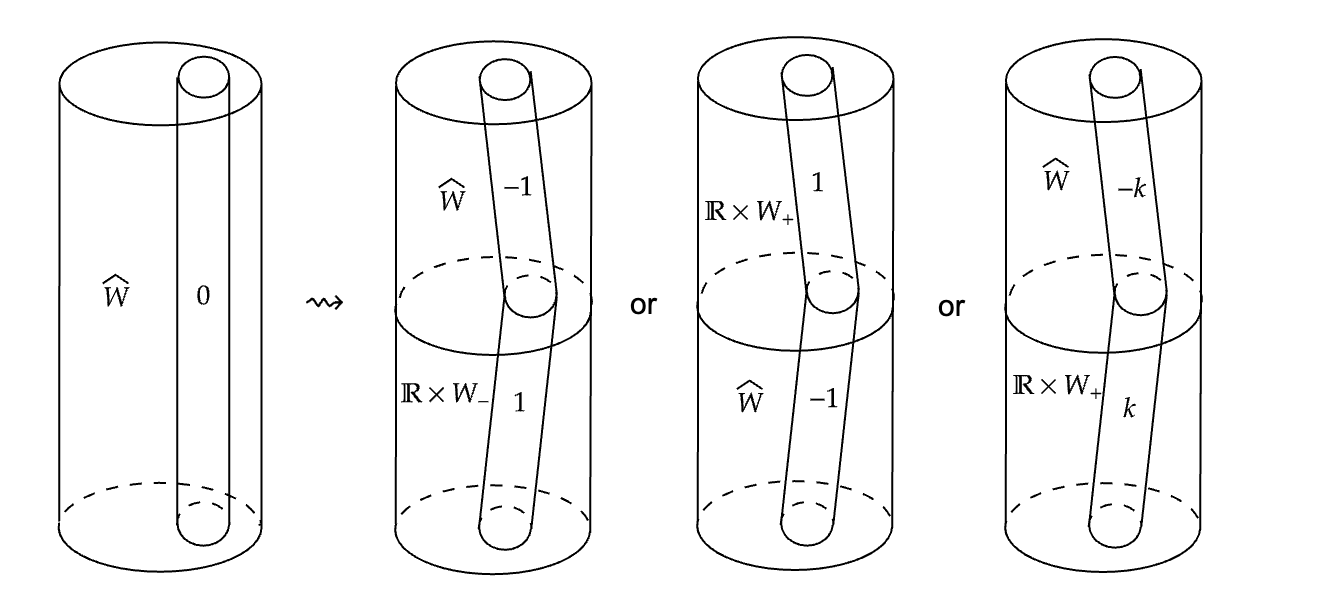
\includegraphics[width=1\textwidth]{images/bao2.png}
  \label{fig:bi14}
\end{figure}
\end{center}
\vspace{-50pt}
For the right most cylinder, we can attach $\mathcal{U}$ to the top half and $\mathcal{M}$ to the bottom half.

For each $\mathcal{U}$, we have a map $\mathcal{S}^{-1}: \mathcal{O}\to [R,\infty)\times M$ and a vector space attached to $\mathcal{O}$ defined by $\ker D_u^*/\mathbb{R} \langle Y \rangle$ where $Y$ comes from variation of $J^2$ and $\mathcal{S}^{-1}(0)$ is the set of curves in $M$ that glue with $\mathcal{U}$.

\section{Semi-Global Kuranishi Structure}

We start with Morse homology case. Let $X$ be a closed manifold, $f: X\to \mathbb{R}$ be a Morse function, $g$ a Riemannian metric, $\phi^t$ the time-$t$ flow of $-\text{grad}_f$, $p\in \text{Crit}(f)$, $\mathcal{D}_p$ be the descending manifold of $p$, and $\mathcal{A}_p$ be the ascending manifold of $p$.

For any $p, q \in \text{Crit}(f)$, 
\[\mathcal{M}(p,q)= \left( \mathcal{A}+q \cap \mathcal{D}_p \right)/\mathbb{R}.
\]

\begin{definition}

An \textbf{interior semi-global Kuranishi chart} is a quadruple $(K, \pi_v: E\to V, \mathcal{L}:V\to E, \psi)$ where
\begin{enumerate}
\item $K\subset M$ is a capacity.
\item $\pi_V: E\to V$ is a finite rank vector bundle of a finite dimensional manifold.
\item $\mathcal{L}$ is a section.
\item $\psi: \mathcal{L}^{-1}(0) \to M$ is homeomorphic onto an open sbuset of $M$ containing $K$.
\item $\dim V - \text{rank} E =\text{vir} \dim\mathcal{M}$
\end{enumerate}

\end{definition}

We order the moduli space $\mathcal{M}_1, \mathcal{M}_2,...$ such that the energy increase. Let
\[
\mathcal{M}_i=\mathcal{M}(p_i, q_i), \qquad E(\mathcal{M}_i)=f(p_i)-f(q_i).
\]
and suppose we have an index tuple $I=(i_1,...,i_n)$ such that $p_{i_m}=q_{i_{m+1}}$. Suppose $S\subset I$ is a subindex tuple. Then $I/S$ is the index tuple obtained by replacing $S$ by an integer which is the index of $\mathcal{M}(p_{s_1}, q_{s_k})$ if $S=(s_1,...,s_k)$, and $\vec{S}\subset I$ is a disjoint union of subindex tuples. We say $I<J$ if there exists $\vec{S} \subset J$ such that $I=J/\vec{S}$.

\begin{definition}

A \textbf{semi-global Kuranishi structure for $\mathcal{M}_1, ..., \mathcal{M}_p$} for any $1\le i \le p$ such that
\begin{enumerate}
\item For each $I$, such that $I/I =i$, $C_I=(\pi_I: E_I \to V_I, \mathcal{L}_: V_I\to E_I, \psi_I: \mathcal{L}_I^{-1}(0) \to M_i )$.
\item For each $I' <I$, we have the restriction inclusion: for $V_{I'I} \subset V_{I'}$ open, we have
   \[\begin{tikzcd}
	& {E_{I'}|_{V_{I'I}}} && {E_I} \\
	\\
	{V_{I'}} & {V_{I'I}} && {V_I}
	\arrow["{{\phi_{I'I}^\#}}", from=1-2, to=1-4]
	\arrow[from=1-2, to=3-2]
	\arrow[from=1-4, to=3-4]
	\arrow["\supset"{description}, draw=none, from=3-1, to=3-2]
	\arrow["{{\mathcal{L}_{I'}}}", curve={height=-18pt}, from=3-2, to=1-2]
	\arrow["{{\phi_{II'}}}", hook, from=3-2, to=3-4]
	\arrow["{{\mathcal{L}_I}}"', curve={height=18pt}, from=3-4, to=1-4]
\end{tikzcd}\]
where the top map is injective and the bottom map is an embedding
\item $\mathcal{L}_I \circ \phi_{I' I} = \phi^\#_{I'I} \mathcal{L}_{I'}|_{V_{II'}}$
\item $(\mathcal{L}_I)_*$ descends to an isomorphism:
        \[
        (\mathcal{L})_I : TV_I/TV_{I\cdot I} \stackrel{\cong}{\longrightarrow} E_I/E_I
        \]
\item Composition of $(\phi_{I'I}, \phi^\#)$ is associative
\item $\mathcal{M}_i = \bigcup_{I, I/I = i} \psi_I(\mathcal{L}_I^{-1}(0))$
\end{enumerate}

\end{definition}

\section{Strata Compatibility}

\begin{definition}

For $I=(i_1,...,i_m)$ define
\begin{align*}
\mathbb{V}_I&=V_{i_1}\times ... \times V_{i_m} \times [R, \infty)^{m-1}, \\
\mathbb{E}_I &= E_{i_1} \oplus ... \oplus E_{i_m}.
\end{align*}
Suppose that $G_I$ a diffeomorphism onto its image, $G_I^\#$ a bundle isomorphism, and $\mathcal{L}_I$ are $C'$-close as $T_1,....,T_{m-1}\to \infty$.

For all $i$, a bundle map satisfies the \textbf{strata compatibility} conditions if the following map commutes
\[\begin{tikzcd}
	{\mathbb{E}_I} && {E_I} \\
	\\
	{\mathbb{V}_I} && {V_I}
	\arrow["{G_I^\#}", from=1-1, to=1-3]
	\arrow[from=1-1, to=3-1]
	\arrow[from=1-3, to=3-3]
	\arrow["{(\mathcal{L}_1, \mathcal{L}_2,..., \mathcal{L}_m)}", curve={height=-18pt}, from=3-1, to=1-1]
	\arrow["{G_I}"', from=3-1, to=3-3]
	\arrow["{{\mathcal{L}_I}}"', curve={height=18pt}, from=3-3, to=1-3]
\end{tikzcd}\]
\end{definition}

Here, the perturbation section is 
\[
\sigma=\left\{G_I: V_I\to F_I \mid I/I = i \right\}
\]
where $\sigma_I$ transverses $\mathcal{L}_I$, $\sigma_I$ is small, the section is compatible with $(\phi_{I'I},\phi_{I'I}^\#)$, and both $\sigma_I$ and $(\sigma_{i_1,i_2,...,i_n})$ are $C^1$-close as $T_1,...,T_{n-1}\to \infty$.

The perturbed moduli space is
\[
Z_i = \coprod_{I/I=i} \mathcal{L}_I^{-1}(\sigma_I)/\sim
\]

\section{Construction of Semi-Global Kuranishi Structures for Cylindrical Contact Homology}

Suppose we have an interior chart $\mathcal{E}\to \mathcal{B}$ and $\overline{\partial}$ on the inverse.

\begin{theorem}

Given any compact $K\subset \mathcal{M}$, there exists an integer and a neighborhood $N(K)\subset B$ and a rank $\ell$ sub-bundle $E\subset \mathcal{E}$ defined over $N(K)$ such that $\overline{\partial}$ transverses $E$ over $N(K)$.

\end{theorem}

\begin{proof}
Pick $\epsilon \gg 0$ small. Find $s_0 \in \mathbb{R}$ such that $\mathcal{A}(u(s-s_0))= \mathcal{A}(\gamma_+)-\epsilon$. Choose $J$ such that $\overline{\partial}_J u = \partial_S u+Au=0$ (where $A$ is a linear self-adjoint operator) is a linear near $\infty$.
\end{proof}

Let $f_i, \lambda_i$ be eigenvectors and eigenvalues of $A$ ordered such that $\lambda_{-2} \le \lambda_{-1} < 0 < \lambda_1\le \lambda_2 \le ...$ and consider
\[
\tilde{f}_j(s,t)=\beta(s)f_k(t)\otimes (\,ds -i\,dt).
\]

Then let $E=\text{span}\{\tilde{f}_1,...,\tilde{f}_\ell\}$. The claim is that $E$ transverses $\overline{\partial}$.  we have $V=\overline{\partial}^{-1}(E)$.

This involves proving the following diagram commutes:

\[\begin{tikzcd}
	{\mathcal{O}_+\oplus \mathcal{O}_-} &&& {\mathcal{O}_{+-}} \\
	\\
	{\mathcal{M}_+ \times \mathcal{M}_- \times [\mathbb{R}, \infty)} &&& V
	\arrow["{G_\#}"', from=1-1, to=1-4]
	\arrow[from=1-1, to=3-1]
	\arrow[from=1-4, to=3-4]
	\arrow["{(0,0)}", curve={height=-24pt}, from=3-1, to=1-1]
	\arrow["G"', from=3-1, to=3-4]
	\arrow["{\mathcal{L}}"', curve={height=18pt}, from=3-4, to=1-4]
\end{tikzcd}\]